\documentclass{article}

\usepackage[
  paperheight=8.5in,
  paperwidth=5.5in,
  left=10mm,
  right=10mm,
  top=20mm,
  bottom=20mm]{geometry}
\usepackage[utf8]{inputenc}

\usepackage{graphicx}
\usepackage{wrapfig}
\usepackage[bottom]{footmisc}
\usepackage{listings}
\usepackage{enumitem}
\usepackage[backend=bibtex]{biblatex}

\usepackage{wrapfig}
\usepackage{ragged2e}

\usepackage{array}
\usepackage[table]{xcolor}
\usepackage{multirow}
\usepackage{booktabs}
\usepackage{hhline}
\definecolor{palegreen}{rgb}{0.6,0.98,0.6}

\usepackage{amsmath}
\usepackage{amssymb}
\usepackage{multicol}
\usepackage{lipsum}
\usepackage{hyphenat}
\PassOptionsToPackage{hyphens}{url}
\usepackage{url}

\usepackage{rotating}

%\usepackage{xeCJK}

%% support use of straight quotes in code listings
\usepackage[T1]{fontenc}
\usepackage{textcomp}
\usepackage{listings}
\usepackage{biblatex}
\lstset{upquote=true}

%% for shrinking space between lines
\usepackage{setspace}

\newcommand*{\affaddr}[1]{#1} % No op here. Customize it for different styles.
\newcommand*{\affmark}[1][*]{\textsuperscript{#1}}
\newcommand*{\email}[1]{\small{\texttt{#1}}}
\newcommand{\tarot}{\textsc{Tarot}}
\renewcommand*\contentsname{\centering Table of Contents}

\renewcommand{\footnoterule}{%
  \kern -3pt
  \hrule width \textwidth height 0.5pt
  \kern 2pt
}

% remove date
\date{}

\usepackage{titlesec}
\titleformat*{\section}{\large\bfseries}
\titleformat*{\subsection}{\normalsize\bfseries}
\titleformat*{\subsubsection}{\normalsize\bfseries}



\addbibresource{reference.bib}

\title{Web Application for Research Paper Management\footnote{\protectCopyright \copyright 2022 by the Consortium for Computing Sciences in Colleges.
Permission to copy without fee all or part of this material is granted provided
that the copies are not made or distributed for direct commercial advantage,
the CCSC copyright notice and the title of the publication and its date appear,
and notice is given that copying is by permission of the Consortium for
Computing Sciences in Colleges.  To copy otherwise, or to republish, requires
a fee and/or specific permission.
}
}
\author{Unknown}

%\author{
%Ratan Lal\affmark[1], Saivivek Reddy  Kusukuntla\affmark[2] \\ 
%Jawahar Reddy Nomula\affmark[3], Nithin Reddy Kumbham\affmark[4]\\
%Abhinav Bellamkonda\affmark[5],Vamsidhar Reddy\affmark[6],\\
%Gopi Krishna Kandimalla\affmark[7] \\
%\affmark[1,2,3,4,5,6,7]School of Computer Science and Information Systems\\
%Northwest Missouri State University\\
%Maryville, MO 64468\\
%\email{rlal@nwmissouri.edu}
%}

\begin{document}
\maketitle

\begin{abstract}
In this paper, we consider a problem to assist researchers for managing research papers read by them. Our broad approach is to develop a web application, where researchers could upload their interested papers with topic, year, title, and technique. Upon uploading a paper, they can read the paper,  write and save comments about the paper. To develop the application, we have used React, which is an open source JavaScript library for creating interactive website and standalone application. For storing users' information and research articles, we have used Firebase database.
\end{abstract}


\section*{Introduction} Different content management systems have been studies, such as, learning management system~\cite{abazi2008development}, content management system~\cite{mooney2008extensible,michelinakis2004open}, course management system~\cite{brooks2006awareness}, Web-based content management system~\cite{dobecki2010web}. In addition, Researchers uses reference management tools~\cite{singh2010mendeley,eapen2006endnote,grolimund2012citation,beel2011docear} for maintaining the history of research papers read by them. Most of available reference website/tools provides researchers to create  bibliographies and citations. Some of them also allow researchers to collaborate with others. Using these tools, users can store, organize and search all available references.
 However, it is hard for the researchers to remember what they have read in the past months and years.
Hence, we focus on developing an application that could assist researchers to read papers online and allow them to write their notes about the paper. Although the application is beneficial to all the researchers, it will be more useful to multidisciplinary investigators. 

In the application, we allows users to upload their interested papers with topic, year, title, and techniques. This helps the researchers to find all their interested papers based on research topic, year, title, and techniques. For each uploaded paper, the application provides an interactive window for the users to read the paper, write comments on the paper. The comments are stored along with time. 

The application consists of two parts, namely, front and back end. For the front-end part, we have developed interactive web pages for the users to register, login, upload and search papers based on one or more criteria, and view a selected paper and write notes/comments about the paper. All the pages have been developed using React. For the back-end part, we have used Firebase to store the uploaded papers and comments. 

\newpage
\section{System Design} In this section, we describe the flow diagram of the application given in Figure \ref{fig:design}. For the application, we have developed the following React components.
\begin{figure}[htp]
	\centering
	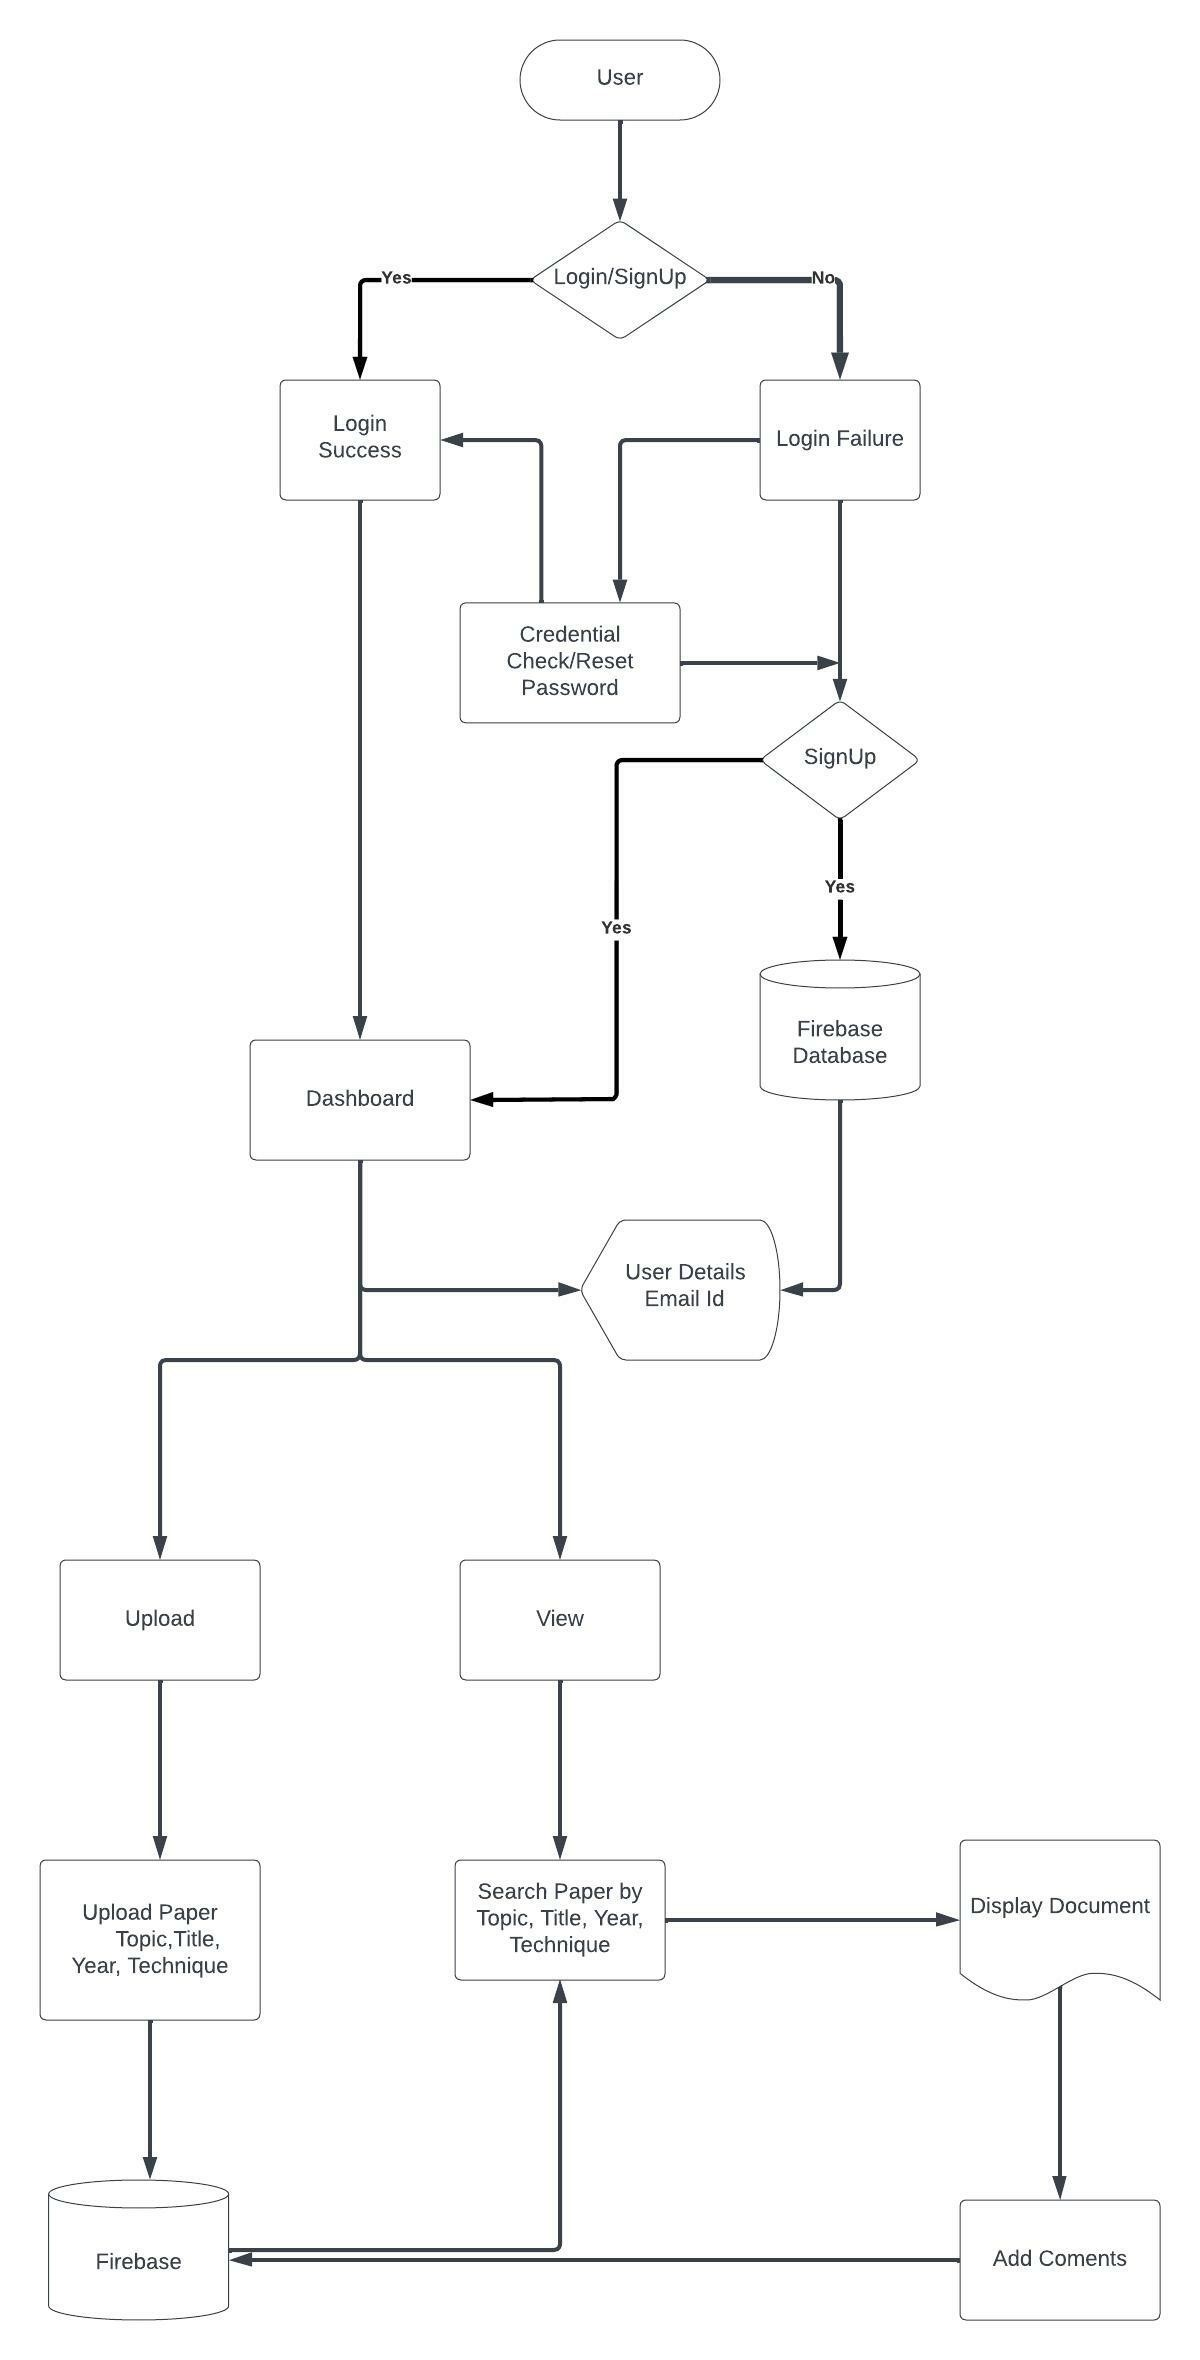
\includegraphics[width=11cm,height=12.5cm]{./images/flow.jpg}
	\caption{Research Content Management}
	\label{fig:design}
\end{figure}
\paragraph{\textbf{Register:}} For the new users, we 
have developed a register component for creating an account on the application shown in Figure \ref{fig:register}. To register, the users have to fill up their information, namely, name, email, and password. 

We also provide another option to users for registering through their google account, that is, if one has a valid Google account saved in his local machine, he/she can register at a glance using the above mentioned feature. The authentication requirements provided by the Firebase are needed to meet like password should be minimum of 6 characters in length and email address should end up with .com. 
\begin{figure}[t]
	\centering
	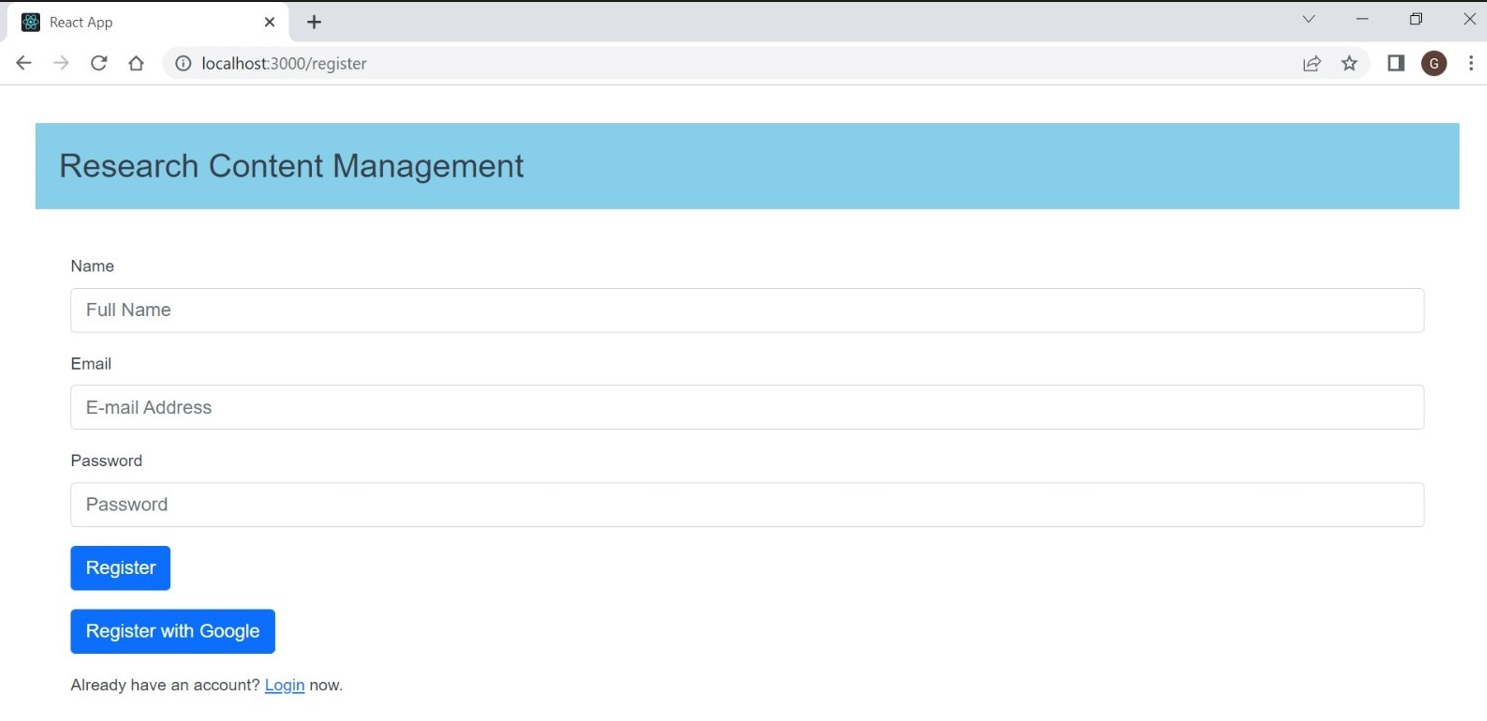
\includegraphics[width=11cm,height=6cm]{./images/register.png}
	\vspace{-0.5cm}
	\caption{Register Page}
	\label{fig:register}
\end{figure}

\paragraph{\textbf{Login:}} For existing users, we have develop a login component shown in Figure \ref{fig:login}.
\begin{figure}[htbp]
	\centering
	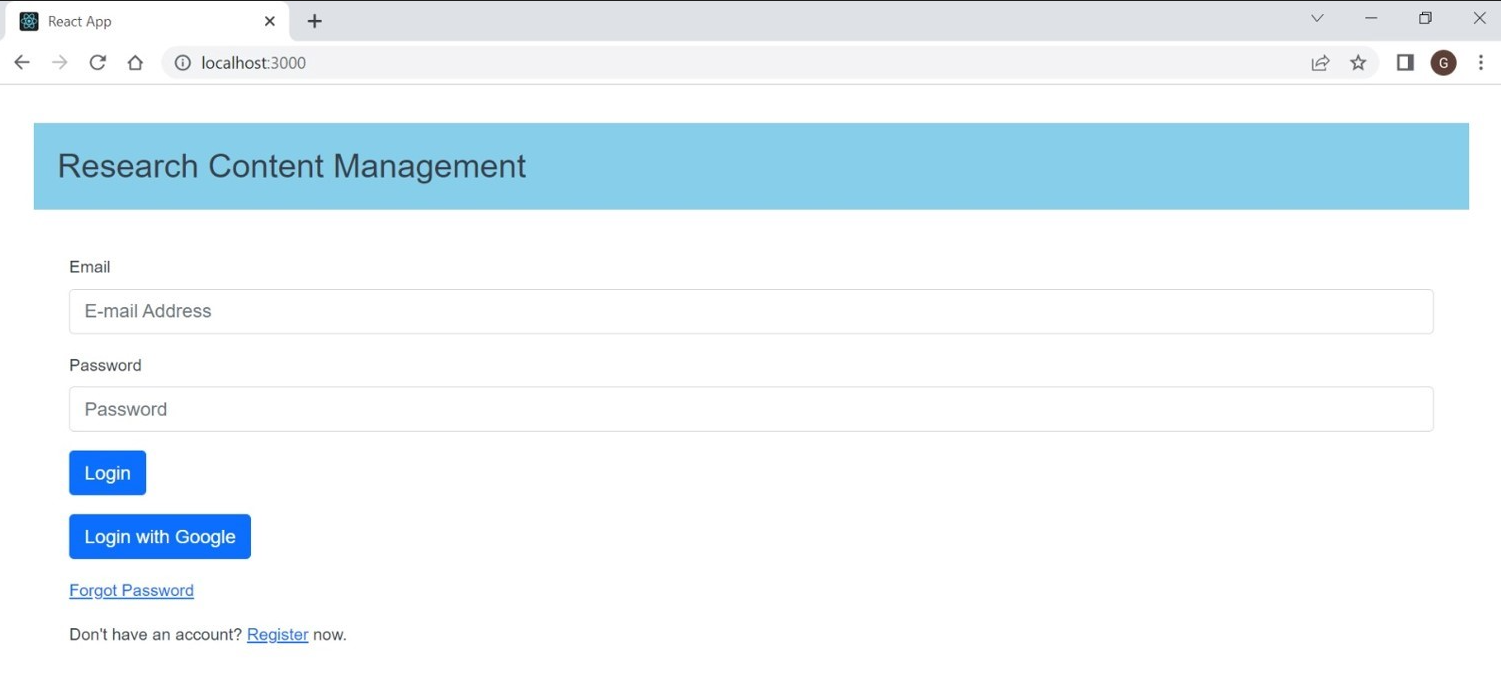
\includegraphics[width=11cm,height=5cm]{./images/login.png}
	\vspace{-0.5cm}
	\caption{Login Page}
	\label{fig:login}
\end{figure}
 Once a user has successfully created/registered an account he/she can login to website using his/her email address and password.
 Alternatively, the user can also login with Google account as we have the option of registering using Google account. If the user forget his/her password, the user can reset the password via  forgot password link, which we provide on the login page. Upon clicking the link, the user has to enter his registered email address in order to reset the password. 

\paragraph{\textbf{Dashboard:}} We have developed a dashboard component for the users to upload, search and view papers upon login. The dashboard consists of website name to the left and the user can see his name, email address and logout button to the right. This dashboard gives the user a quick glance of user details.

\paragraph{\textbf{Upload:}} We have developed an upload component for the users to upload their interested papers shown in Figure \ref{fig:upload}.This page allows a user to upload a research paper on which he/she is currently working or previous research papers which he/she worked on. For making the uploaded paper unique, there are several factors taken into consideration. The paper which user wants to upload should be of pdf format, should choose a topic for the paper, year of publishing for the paper, title of the paper, and finally technique of the paper. By choosing the above metrics, each paper represents unique. When the user clicks on submit button given in Figure \ref{fig:upload}, the paper is directly uploaded to the Firebase server which later can be accessed.
\begin{figure}[h]
	\centering
	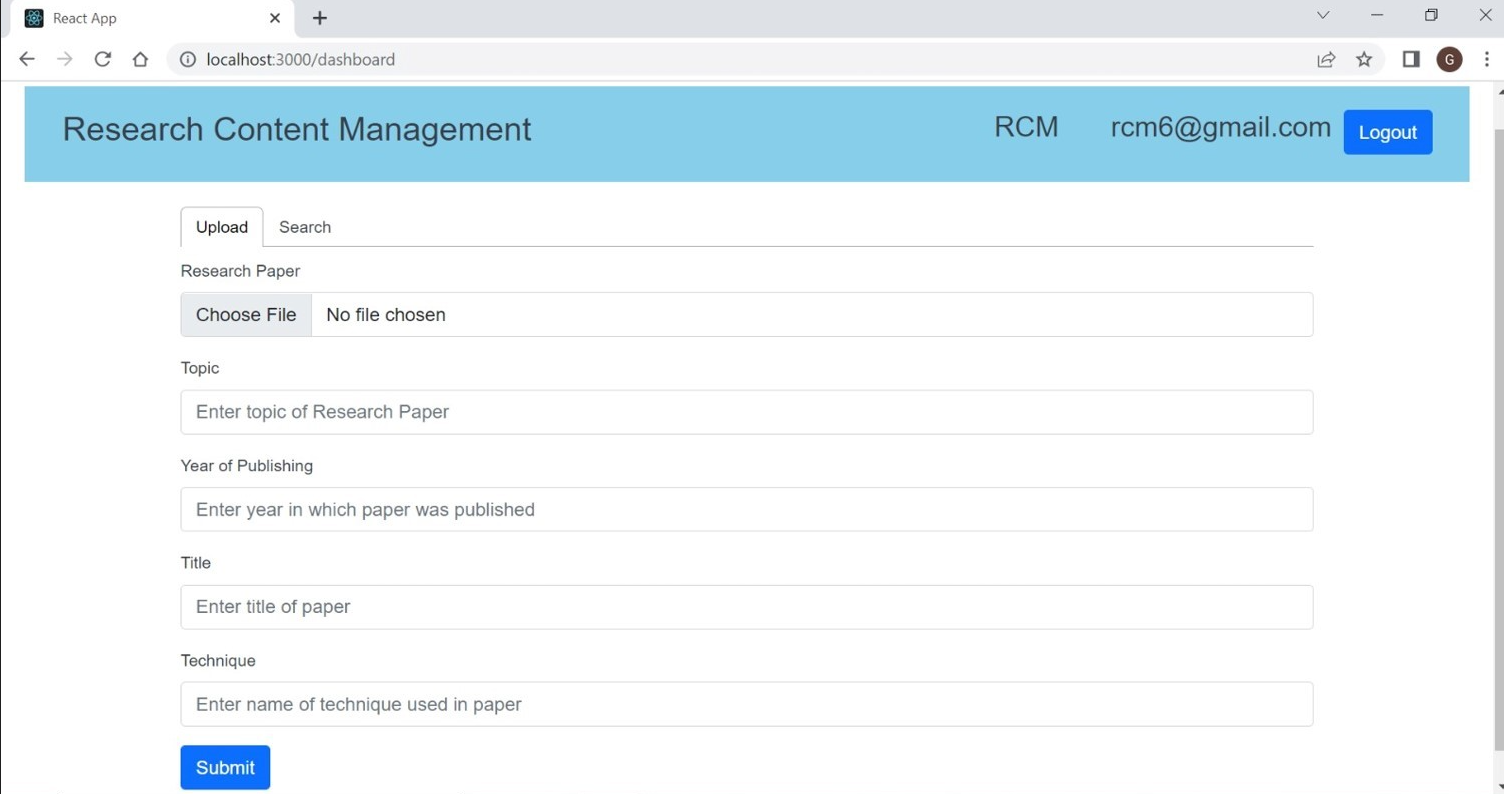
\includegraphics[width=11cm,height=6cm]{./images/upload.png}
	\vspace{-0.5cm}
	\caption{Upload Page}
	\label{fig:upload}
\end{figure}

\paragraph{\textbf{Search:}} Upon login, a user can search interested papers that have been already uploaded by him/her. For this, we have developed a search component. It uses the Firebase database finding papers based on topic, title, year or technique. Upon entering these key values, the user has to enter the search button shown in Figure \ref{fig:search}. Upon clicking on search button, the component interacts with the Firebase database and find all matching papers stored in the Firebase database. For this, we have implemented effective 
search technique.
\begin{figure}[h]
	\centering
	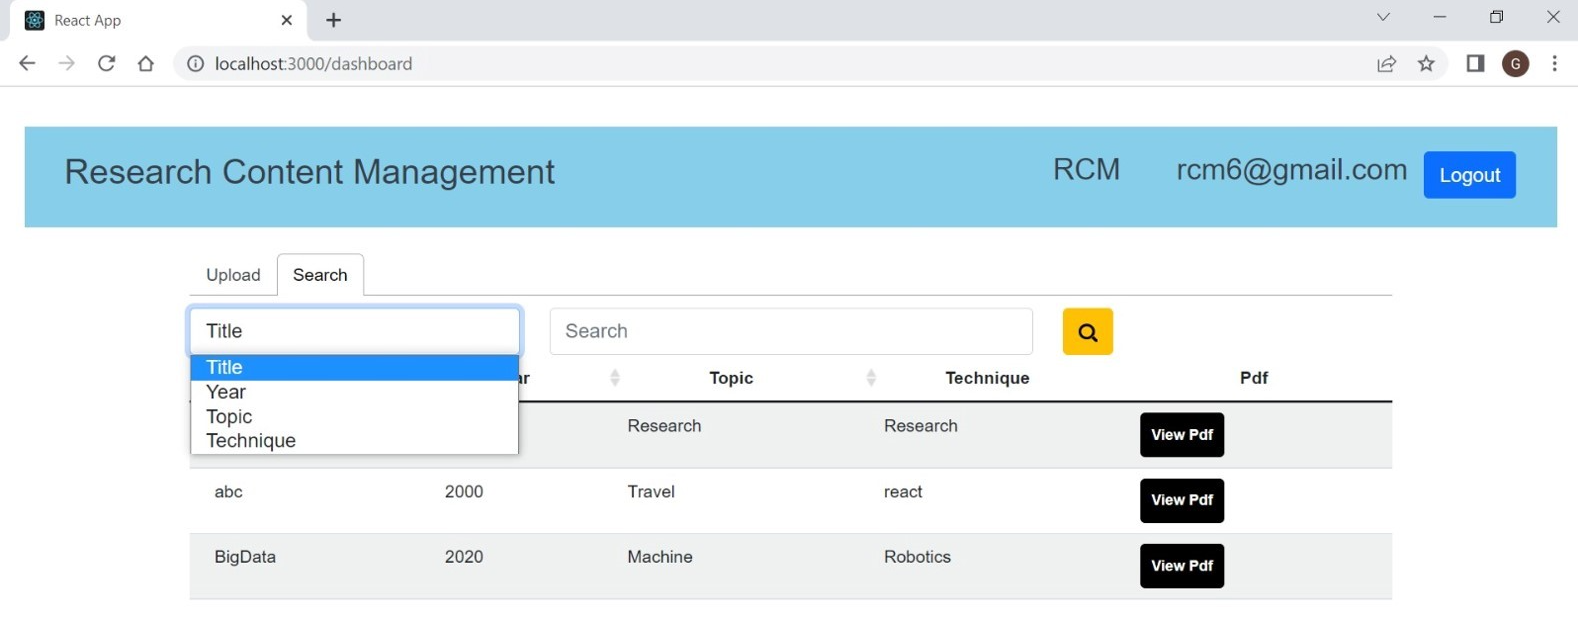
\includegraphics[width=11cm,height=6cm]{./images/search.png}
	\vspace{-0.5cm}
	\caption{Search Page}
	\label{fig:search}
\end{figure}

\paragraph{\textbf{View:}} Upon searching papers, the user may wish to view/read a specific paper. For this, we have developed view component shown in Figure \ref{fig:view}. After search operation, there is a view button on each matched paper. When the user clicks on a specific paper, view component will help the user to read/view the paper along with comments facility. If the user wants to add comments for the paper, he/she needs to enter the note in comments box and to click on post comment button. Then, the comment for the paper will be stored in database with timestamp. When user clicks on show comments button, the comments which are posted for the paper is displayed as list with the timestamp.
\begin{figure}[h]
	\centering
	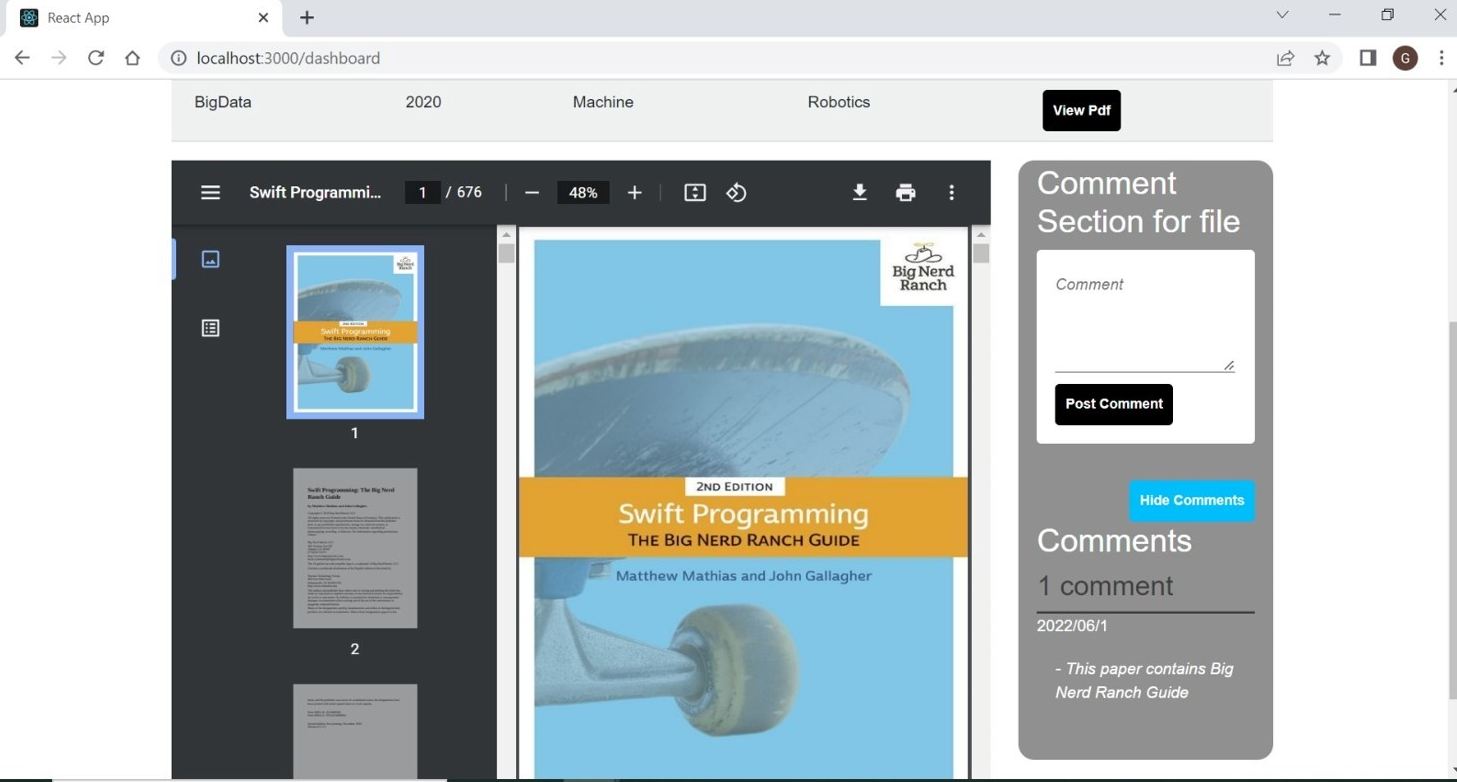
\includegraphics[width=11cm,height=6cm]{./images/view.png}
	\vspace{-0.5cm}
	\caption{Search Page}
	\label{fig:view}
\end{figure}






\section{Features} In this section, we will provide the details about certain features of the application.

\paragraph{\textbf{Performance}} The application is built in React and is integrated with Firebase.The performance of the application is fast and user-friendly. Users can navigate between different sections of the application with ease.

\paragraph{\textbf{Reliability}} The application delivers correct output to the user from start to end. Users can retrieve any stored paper with ease and add comments for further review and update it accordingly. The application delivers what it needs to perform and asks inputs accordingly so that it can work accordingly.

\paragraph{\textbf{Availability}} The application is free to use for any users. As the application is designed keeping in view of various users where they can store their research work and retrieve for further use. Users can create an account and login with their credentials, upload and retrieve papers for further use.

\paragraph{\textbf{Security}} The application is protected with authentication provided by Firebase where it doesn’t allow other users to use some others account until and unless the login credentials are misused. Firebase has various inbuilt authentication steps to register or login just by enabling and using the features in code.

\paragraph{\textbf{Portability}} Currently, the application is designed as web application. The application runs on server side so there is no restriction for any systems other than mobile devices.



\section{Implementation of the Application} In this section, we provide the details about the implementation and execution of the application.

\paragraph{\textbf{Creating a new React project}} First, we have created a React project via the following steps:
\begin{itemize}
	\item A new React project can be created by using command
	``npx create-react-app my-app" where my-app is your app name.
	\item Developer can use any IDE for developing a react application.
	\item After the successful execution of the above command, a basic react application will be created.
\end{itemize}

\paragraph{\textbf{Managing package.json}} We use package.json for storing information about the application. The package.json file consists of metadata where the file includes all the details about the application that includes application name, version, dependencies installed and their version and debugging dependencies.

\paragraph{\textbf{Components}} Components are building blocks for the React component. A React application can have many components where a developer writes clean and efficient code in a component and embed the component to a main file.There are two types of components in React JavaScript, namely, functional and class component.

\paragraph{\textbf{Adding Database to React Application}} To our react application we have chosen the Firebase as primary database where our application has authentication, storage and managing the users. To make the Firebase in sync with react application, a developer needs to create a project in the Firebase and choose the application which he/she needs to develop so that the Firebase provides a snippet code which is ready to use. We use the provided snippet by the Firebase in our react application by creating a new .js extension file. By using above file we can import the Firebase functionalities to our react application.

\paragraph{\textbf{Embedding Components to App.js}} All the components which were created in React application needs to embed in main file i.e., App.js so that whenever react application call index.js, it  renders App.js in strict mode and all the components in App.js will be displayed whenever application is run. 

\paragraph{\textbf{Running React Application}} After adding all the components to App.js the application needs to be run on the server side. React application can be run on the server side using command ``npm start" and the application can be viewed on localhost:3000. In order to run the application some of the dependencies need to be installed and they can be installed by running the below commands in VS code terminal.
\begin{itemize}
	\item 	npm install react-scripts –save
	\item 	npm install -S react-router-dom
	\item 	npm install --save react-firebase-hooks
\end{itemize}





\section{Conclusion} In this paper, we have developed a web application to assist researchers for the effective management of the articles read by them. We have developed the application using React and Firebase. The application is easy to use and all the interaction pages are user friendly. In the future, we plan to add more features, such as, word documents, automatic detection of topic, title, and technique. 


\medskip

\printbibliography

\end{document}
